\documentclass[11pt]{amsbook}

\usepackage{../HBSuerDemir}	% ------------------------

\usepackage{tabto}
\usepackage{wrapfig}
\begin{document}

% ++++++++++++++++++++++++++++++++++++++
\hPage{b1p2/314}
% ++++++++++++++++++++++++++++++++++++++

\noindent done, dividing all terms of the fraction by A.\newline
\indent If the polar axis is rotated by an angle $\alpha$, the last equation 
becomes (dropping the primes):
\[
    r = \frac{D}{A+B_{1}cos(\theta-\alpha)}
\]
which is of the form

\[
    r = \frac{D}{A+Bcos(\theta)+Csin(\theta)} \quad (A \neq 0)
\]\\*

\noindent where \\
\[
B = B_{1}cos(\alpha),\
C=B_{1}sin(\alpha),\
B^{2}+C^{2}=B_{1}^{2},\
tan(\alpha) = C/B
\]

\[
 e = \frac{\sqrt{B^{2}+C^{2}}}{A}
\]
\begin{exmp}
Identify and sketch the following conics: 
\footnote{Identity is replaced by Identify}
\end{exmp}


a) $r= \frac{6}{2-cos(\theta)}$ \tab b) $r  = \frac{10}{2+3sin(\theta)}$ \newline

\begin{wrapfigure}{r}{5.5cm}
	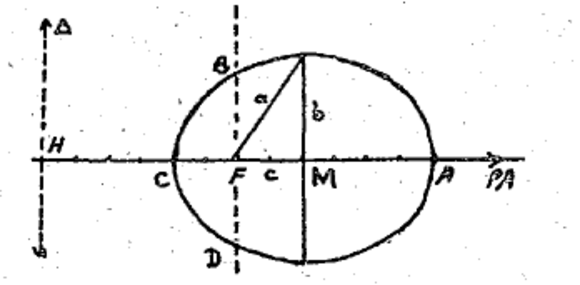
\includegraphics[width=5.5cm]{images/b1p2-314-fig01}
\end{wrapfigure}


\underline{Solution}.
\newline
\newline
\indent a)\ $e = \frac{1}{2}<1:\ \text{Ellipse}.\\
\indent ep = 6/2 \rightarrow p = 6.\\
\indent \text{Intercepts}:\\
\indent A(0, 6),\quad B(\pi/2, 3)\\
\indent C(\pi, 2),\quad D(-\frac{\pi}{2}, 3)\\
\indent 2a = \hAbs{CA} = 8 \rightarrow a=4\\$
\indent$ c=ae=2,\quad b=\sqrt{16-4}=2\sqrt{3}\\
\indent \hAbs{MH}=a/e=8,\quad \hAbs{MF}=ae=2$\\
\footnote{16-4 is replaced by $\sqrt{16-4}$}

\begin{wrapfigure}{r}{5.5cm}
	\vspace{-1.0cm}
	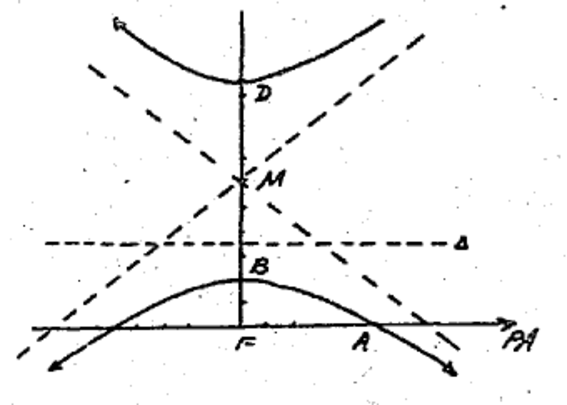
\includegraphics[width=5.5cm]{images/b1p2-314-fig02}
\end{wrapfigure}

b)\ $e = \frac{3}{2} > 1: \text{Hyperbola}.\\
\indent ep = 5 \rightarrow p = 10/3\\
\indent \text{Intercepts}:\\
\indent A(0, 5),\quad B(\pi/2, 2)\\
\indent C(\pi, 5),\quad D(-\frac{\pi}{2}, -10)\\
\indent \text{Asymptotes}: r \rightarrow \infty$
\footnote{Figures are transformed from pdf to png using inkscape}

\end{document}  

